\chapter{Serverlist}
\label{chap:serverlist}

In this chapter, we discuss the interaction between the game client and masterserver to retrieve a list of gameservers.

\begin{figure}[h]
\centering
\input{tikz/overview-cms}
\caption{Focus on interaction between game client and masterserver.}
\label{fig:overviewcms}
\end{figure}

\section{List transfer}
In the previous chapter, we discussed how heartbeats sent to the masterserver result in a complete list of online gameservers at the side of the masterserver. In this chapter we discuss how the list of gameserver addresses is transferred to the game client as seen in step (2) in figure \ref{fig:overviewcms}. The request is initiated when the user opens the \emph{server browser} in the game environment (further discussed in chapter \ref{chap:status}). The serverlist merely contains a list of IP-addresses and query ports. When the client requests the serverlist from the masterserver, the list of addresses is transmitted.

In contrary to heartbeats, which are sent over UDP, the serverlist is sent over TCP. The integrity of the rather large serverlist is important and must be preserved during the transfer, usually split over multiple packets. To protect the data, GameSpy preferred the slower but more reliable TCP transfer for this part in the process.


\section{Procedure}
As soon as the user requests the serverlist, the client initiates a request to the masterserver by opening a connection to one or more of the configured masterservers. In listing \ref{ls:gs0servlist}, the exchange of the GameSpy protocol is detailed. After a TCP connection is established, the masterserver opens the exchange with a request for the basic client information (gamename, game version) and authentication via the \emph{secure} challenge that was also used by the masterserver to authenticate heartbeats (line 1).

The client returns the basic game information and generated validate keyword in the same packet to the masterserver. As the client and the masterserver both possess the game cipher and secure keyword, as well as the gamename from the masterserver's request for basic client information, both the masterserver and the client can calculate the correct \emph{validate} keyword to complete the authentication (lines 2 and 3).
\lstinputlisting[caption={Example of the GameSpy protocol message formatting.},
                 stepnumber=1, 
                 xleftmargin=1.8cm,
                 xrightmargin=1.8cm,
                 label={ls:gs0servlist}
                ]{lst/gs0serverlist.txt}
The client then proceeds with requesting the serverlist and the format in which the client would like to receive this information (line 4 or 5). If the client properly authenticated with the secure/validate keyword, the masterserver will start sending the serverlist over multiple packets. This could be a plaintext list, or compressed list as described in the following section (line 6). The masterserver appends the {\tt final} keyword to serverlist, to indicate that the last address has been received. Immediately after sending the last packet, the masterserver closes the TCP connection.

The client will continue to receive data until the {\tt final} keyword has arrived. If due to network disruption the {\tt final} does not arrive, the client will attempt to receive until a timeout occurs. The addresses that are intact are processed for display to the user, missing addresses are ignored. Many games do \emph{not} throw an error or warning when the received list was incomplete, but fail silently. 

\begin{figure}[H]
\centering
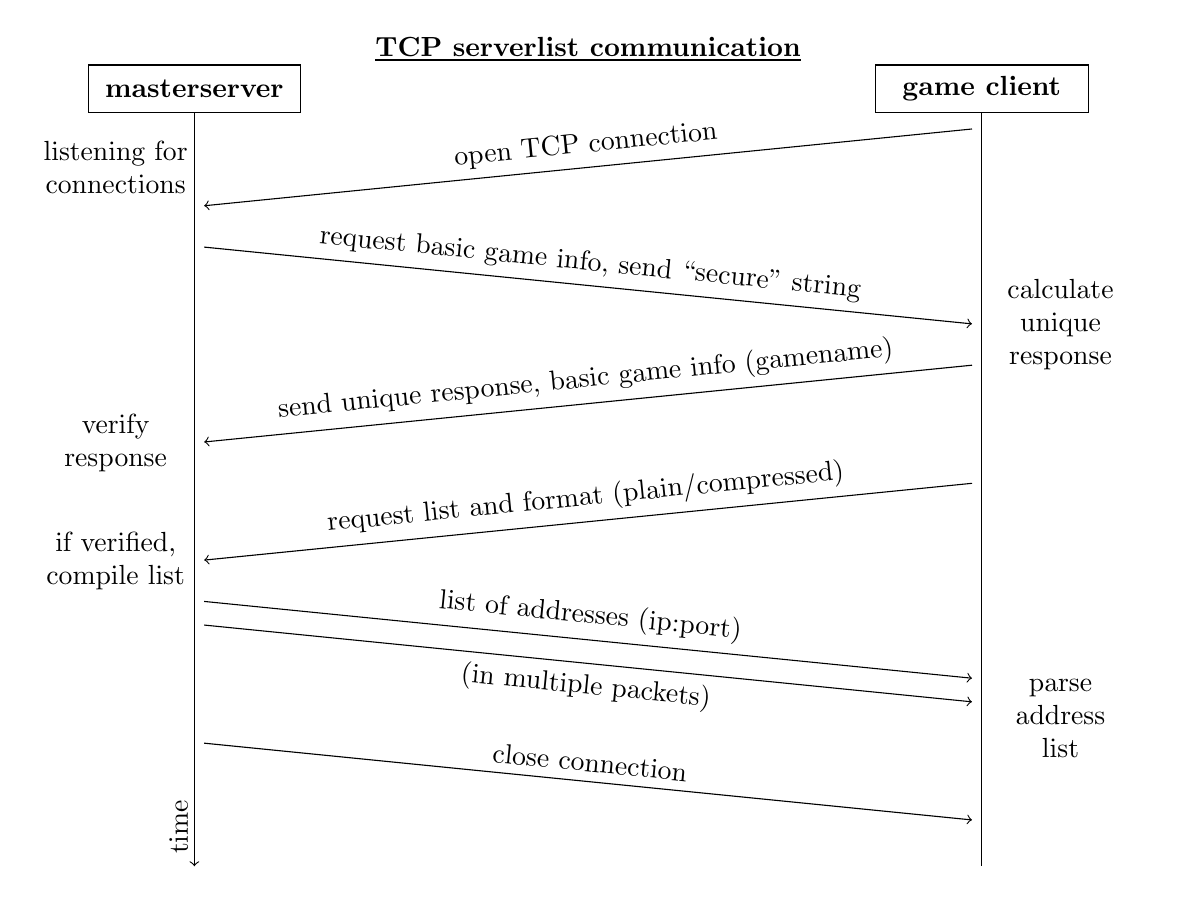
\begin{tikzpicture}

% figure title
\node[rectangle] at (5, 10.5) (title) {\underline{\bf TCP serverlist communication}};

% ms and gc, top
\node[draw, rectangle, minimum height=0.6cm, minimum width=2.7cm] at (0,  10.0) (mstop) {\bf masterserver};
\node[draw, rectangle, minimum height=0.6cm, minimum width=2.7cm] at (10, 10.0) (gctop) {\bf game client};

% open connection
\node at (10,  9.5) (gcoc) {};
\node at ( 0,  8.5) (msoc) {};
\node at (-1,  9.0) (mslisten) [text width=2cm, text centered]{listening for\\connections};
\draw[->] (gcoc) -- (msoc) node[midway, above, sloped] {open TCP connection};

% secure
\node at ( 0,  8.0) (msse) {};
\node at (10,  7.0) (gcse) {};
\node at (11,  7.0) (gcsecure) [text width=2cm,text centered]{calculate unique\\ response};
\draw[->] (msse) -- (gcse) node[midway, above, sloped] {request basic game info, send ``secure'' string};

% validate        
\node at (10,  6.5) (gcva) {};
\node at ( 0,  5.5) (msva) {};
\node at (-1,  5.5) (msvalidate) [text width=2cm,text centered]{verify\\ response};
\draw[->] (gcva) -- (msva) node[midway, above, sloped] {send unique response, basic game info (gamename)};

% list request
\node at (10,  5.0) (gcli) {};
\node at ( 0,  4.0) (msli) {};
\node at (-1,  4.0) (mslist) [text width=2cm, text centered]{if verified, compile list};
\draw[->] (gcli) -- (msli) node[midway, above, sloped] {request list and format (plain/compressed)};

\node at ( 0,  3.5) (msl1) {};
\node at (10,  2.5) (gcl1) {};
\draw[->] (msl1) -- (gcl1) node[midway, above, sloped] {list of addresses (ip:port)};

\node at ( 0,  3.2) (msl2) {};
\node at (10,  2.2) (gcl2) {};
\node at (11,  2.0) (gcparse) [text width=2cm, text centered]{parse\\address\\list};
\draw[->] (msl2) -- (gcl2) node[midway, below, sloped] {(in multiple packets)};

% close connection
\node at ( 0,  1.7) (mscc) {};    
\node at (10,  0.7) (gccc) {};    
\draw[->] (mscc) -- (gccc) node[midway, above, sloped] {close connection};

% ms and gc, bottom, vertical lines
\node at ( 0, 0) (msbot) {};
\node at (10,  0.0) (gcbot) {};
\draw[->] (mstop.270) -- (msbot.90) node[at end, xshift=-0.2cm, yshift=0.5cm, rotate=90] {time};
\draw (gctop.270) -- (gcbot.90) {};

\end{tikzpicture}

\caption{TCP interaction between the masterserver (left) and game client (right) over time.}
\label{fig:client}
\end{figure}

\section{Compressed serverlist}
Gameserver addresses are usually expressed as an IP-address and query port with a colon ({\tt :}) as separator in a plaintext string. The length of this string is up to 21 characters, with a 4- or 5-digit query port as seen in the addresses at line 6 in listing \ref{ls:gs0servlist}. To separate multiple addresses, the {\tt ip} keyword was added for every new address in the list, adding another 4 characters to the plaintext address. Every character requires a single byte to transfer. In the time that the GameSpy protocol was drafted, bandwidth was scarce. With more than two thousand servers during its popular period, a serverlist for Unreal Tournament could easily be $50,000$ characters large and take several seconds to transmit on a dial-up connection.

To reduce the size of the data stream, the \emph{compressed} serverlist was provided as alternative. By specifying the {\tt cmp} value for the {\tt list} keyword (line 5), the masterserver would send a compressed serverlist where the gameserver addresses were not sent as plaintext, but as byte values. 

A single byte can hold $2^8$ or 256 values. With the inclusion of the zero, that leads to a value range between 0 and 255, including both values. An IP-address consists of four octets (groups of numbers) with the values 0 to 255, joined by periods. Conveniently, every individual octet can fit inside a single fixed-length byte, despite the lexical length being two (e.g. $99$) or three (e.g. $101$) digits. As we know that every new byte is a new octet, it is no longer necessary to join the octets by periods in their text representation. 

\begin{table}[h]
\centering
\begin{tabular}{ |c|c|c|c |c|c|c| c |c|c|c| c |c|c|c| c |c|c|c| c |c|c|c|c|c|c| }
\hline
\textbackslash&i&p&\textbackslash&2&5&5&.&2&5&5&.&2&5&5&.&2&5&5&
:&1&2&\multicolumn{2}{|c|}{5}&5&6\\
\hline
\multicolumn{4}{|c|}{} & 
\multicolumn{3}{|c|}{0xFF}& &
\multicolumn{3}{|c|}{0xFF}& & 
\multicolumn{3}{|c|}{0xFF}& & 
\multicolumn{3}{|c|}{0xFF}& & 
\multicolumn{2}{|c}{0x31}& &  % dirty fix: no left cell wall to create "half" a cell below the 5
\multicolumn{3}{|c|}{0x0C}\\
\hline
\end{tabular}
\caption{Data allocation in a gameserver address (every cell represents 1 byte).}
\label{tab:plaintextip}
\end{table}

The query port consists of a number larger than 255 and can therefore not be represented with a single byte. The concept of splicing the query port number into two new numbers is difficult to grasp when we consider the decimal counting system. Therefore we make a detour through the hexadecimal counting system: a single hexadecimal digit can hold 16 values, ranging {\tt 0x0-0xF} or 0--15\footnote{to avoid confusion between different counting bases, we use the prefix {\tt 0x} for hexadecimal numbers. This prefix holds no numerical value. The first two digit in the value {\tt 0x1E62} is {\tt 1E} and not {\tt 0x}.}. Two hexadecimal digits can hold the values between 0x00 and 0xFF or 0--255. With the understanding that two hexadecimal digits can be represented exactly in one single byte, we can now express any number larger than 255 in pairs of hexadecimal digits and thus in multiple bytes.

The query port is an \emph{unsigned short integer} and requires 2 bytes to be represented. The query ports 7778 and 12556 can now be represented as {\tt 0x1E62} and {\tt 0x310C}, where the first byte holds the value {\tt 0x1E} and the second byte {\tt 0x62}. In table \ref{tab:plaintextip} we represented the same IP-address as plaintext (top) and hexadecimal values (bottom), where every occupied table cell is a byte. As seen, the bottom row requires significantly less bytes to store the same data.

Earlier we derived that a plaintext gameserver address with {\tt ip} key prefix can occupy up to 25 characters/bytes. With the hexadecimal representation, we compressed the same address to a fixed length of 6 bytes, which means that the same Unreal Tournament serverlist could now be compressed into a $12,000$-byte data string, a reduction of more than two-thirds of the original plaintext data transfer.
